\documentclass[12pt]{article}		
\usepackage{graphicx}		
\usepackage{tikz}
\usepackage{verbatim}
\usepackage{mathtools}
\usepackage{amsmath}
\usetikzlibrary{arrows,shapes}
\setlength{\oddsidemargin}{.1in}
\setlength{\textwidth}{6.3in}	 
\setlength{\textheight}{8.9in}	
\setlength{\topmargin}{-.5in}

\begin{document}		

\section*{MEET TEEM MatLAB Project \hfill  Spring 2019}
\author*{Alex Gonzalez, Ben Harker, and Kyle Wahlberg}
\vspace{.3in}	

\subsection*{Abstract}
We started this project with a dream, a dream of meat on the grill and summer nights. That dream turned into us sitting, staring at a computer screen, longing for our code to compile. Our initial idea was to model how different kinds of meat cook on different kinds of surfaces, using the numerical methods that we learned in class about FTCS, Heat Advection, and some kind of Graphical User Interface.


\subsection*{Procedure and Problem Statement}
For our project we wanted to model the grilling and searing of different meats using diffusion equations for conduction and convection. We began this project with the FTCS method. The meat starts at a fixed temperature (42$^o$F) as if it had just been taken out of the fridge. Heat is then applied to the meat at a constant temperature (though differing in method) for as long as it takes the meat to reach optimal ``doneness". All of this showed on our GUI that the user could interact with to select different options for cooking, meat type, tempreture, and other variables. The GUI is shown below in Figure \ref{GUI}:

\begin{figure}[htb] % GUI
\label{GUI}
\begin{center}
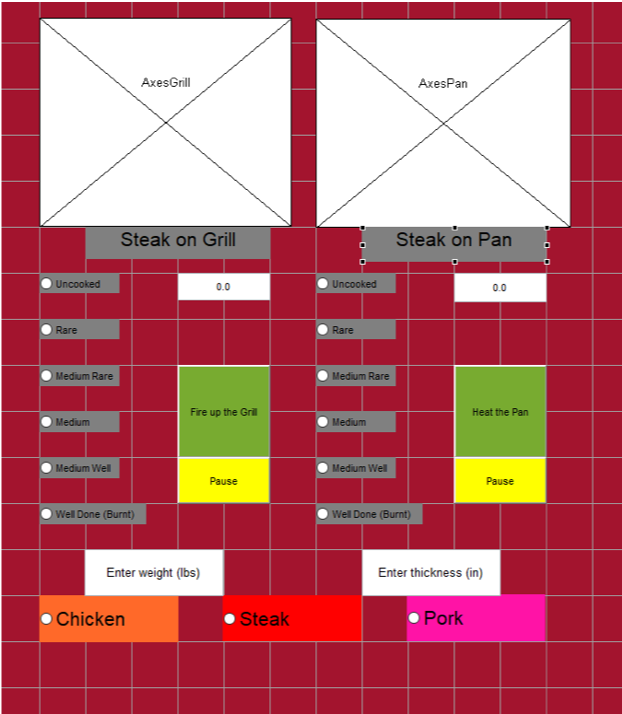
\includegraphics[keepaspectratio=true, width=6.5in, height=3.5in]{gui.png}
\caption{MATLAB Project Graphical User Interface}
\end{center}
\end{figure}

%%%%%%%%%%%%%%%%%%%%%%%%%%%%%%%%%%%%%%%%%%%%%%%%%%%%%%%%%%%%%%%%%%%%%%%%%%%%%%%%%%% ~~~~~~~ Code Portion ~~~~~~~~~ %%%%%%%%%%%%%%%%%%%%%%%%%%%%%%%%%%
%
% Elaborate a bit on what went into making the GUI and some of the code and logic behind it
%
%
\begin{figure}[htb] % code 1 screenshot
\label{code1}
\begin{center}
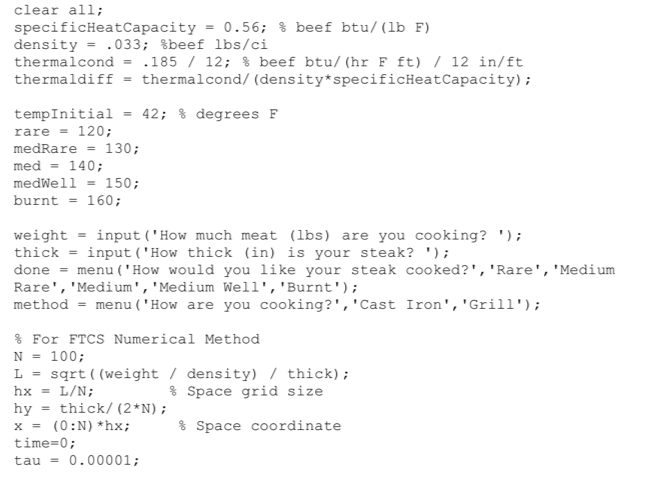
\includegraphics[keepaspectratio=true, width=6.5in, height=2.5in]{code1.png}
\caption{MATLAB code screenshot 1 (see appendix for more)}
\end{center}
\end{figure}

\begin{figure}[htb] % code 2 screenshot
\label{code2}
\begin{center}
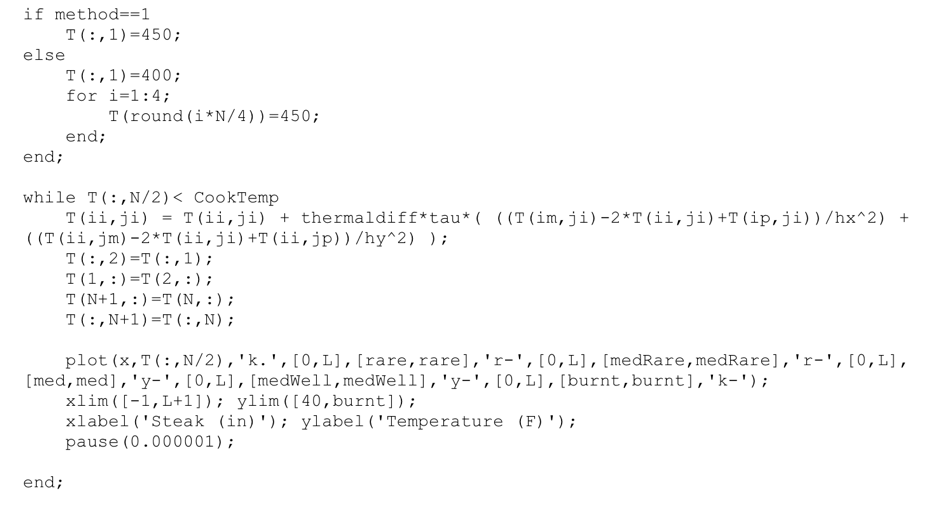
\includegraphics[keepaspectratio=true, width=6.5in, height=2.5in]{code2.png}
\caption{MATLAB code screenshot 2 (see appendix for more)}
\end{center}
\end{figure}

%
%
%
%%%%%%%%%%%%%%%%%%%%%%%%%%%%%%%%%%%%%%%%%%%%%%%%%%%%%%%%%%%%%%




%%%%%%%%%%%%%%%%%%%%%%%%%%%%%%%%%%%%%%%%%%%%%%%%%%%%%%%%%%%%%%%%%%%%%%%%%%%%%%%%%%% ~~~~~~~ Math Portion ~~~~~~~~~ %%%%%%%%%%%%%%%%%%%%%%%%%%%%%%%%%%
%
% More math stuff here? 
%
%
%
To get us a starting point with some of the math that goes into the heat energy transfer to meats, we found two papers, one a master's thesis and the other a doctoral. From these papers we got the equations for conduction, convection, and radiation. Radiation is quite complicated to model, and less important than conduction or convection, so we did not attempt to model it. Conduction and convection seemed straightforward enough, however we ran into some issues.

We realized that the steady state conductivity equations we received from the paper are exactly that, steady state. In our case this means that the heat transfer wouldn't stop until the meat reached the same temperature as the grill, which is quite beyond the ideal medium rare. So after much heartache, we returned to the FTCS method. Additionally, the FTCS method is time dependent, as is the cooking of meat, which lines up quite nicely. 

To use a lot of these equations, we needed some general information about meat. Below are some of the constants and variables we used in our program:

\[
K = 0.185\; \frac{\textrm{BTU}}{\textrm{hr ft}^o\textrm{F}} 
\]\[
C = 0.56\; \frac{\textrm{BTU}}{\textrm{lb} ^o\textrm{F}} 
\]\[
\rho = 0.033 \;\frac{\textrm{lb}}{\textrm{ci}}
\]\[
\textrm{So... } \textbf{k} = \frac{k}{c \;\rho} = 0.834 \;\frac{\textrm{in}^2}{\textrm{hr}}
\]

We also found a table that gave us some information about different kinds of meats we would be grilling (Figure \ref{dataTable}):

\begin{figure}[h!] % data table about meat stuff
\label{dataTable}
\begin{center}
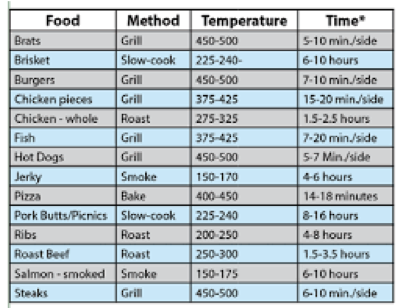
\includegraphics[keepaspectratio=true, width=6.5in, height=2.5in]{dataTable.png}
\caption{MATLAB Project Graphical User Interface}
\end{center}
\end{figure}

%
%
%%%%%%%%%%%%%%%%%%%%%%%%%%%%%%%%%%%%%%%%%%%%%%%%%%%%%%%%%%%%%%



\subsection*{Results}
We had the user input weight of meat, thickness, desired doneness, and then they could select pan or grill. For the pan, we had a constant bottom temperature of 450 $^\textrm{o}$F, and insulated boundaries for the other three sides. On the grill, we had four grates at 450 $^\textrm{o}$F, and the rest at 400$^\textrm{o}$F. This is based off general information that often air temps in grills are less than the actual fire or grate temperature. We also assumed insulated boundaries for the sides and top of the grill
. 
Once all the data was entered, we used the 2D FTCS method to calculate the next temperature given its surroundings. See the appendix for samples of code. We used N=100 steps, but this could easily changed for faster computation or more accuracy. The plot then showed the temperature at the halfway thickness point rising, stopping at the desired temperature. At this point in real life, we would flip the meat and repeat for the same amount of time of the other side. We also included a timer to show how long the meat would take to cook. These times were fairly accurate, however definitely idealized somewhat given we assumed no heat loss to surrounding air, constant temperature and density, and ignored more complex methods of heat transfer.





\subsection*{Appendix}
% We can toss our code and references to our sciency papers here too

%%%%%% Appendic code for the MATLAB code %%%%%%%%%%%%%%%%%%

%%%%%%%%%%%%%%%%%%%%%%%%%%%%%%%%%%%%%%%%%%%%%%

\begin{verbatim}
% matlabProject.m
% Alex Gonzalez, Ben Harker, Kyle Wahlberg
% Due: 5.14.19

%% Set some Variables
% Temperatures
clear all;
specificHeatCapacity = 0.56; % beef btu/(lb F)
density = .033; %beef lbs/ci
thermalcond = .185 / 12; % beef btu/(hr F ft) / 12 in/ft
thermaldiff = thermalcond/(density*specificHeatCapacity);                         %kappa value for FTCS

tempInitial = 42;                     % degrees F
rare = 120;
medRare = 130;
med = 140;
medWell = 150;
burnt = 160;

weight = input('How much meat (lbs) are you cooking? ');
thick = input('How thick (in) is your steak? ');
done = menu('How would you like your steak cooked?','Rare','Medium Rare','Medium','Medium Well','Burnt');
method = menu('How are you cooking?','Cast Iron','Grill');                            %User inputs in lieu of GUI

% For FTCS Numerical Method
N = 100;                       
L = sqrt((weight / density) / thick);
hx = L/N;                                     % Space grid size
hy = thick/(2*N);
x = (0:N)*hx;                               % Space coordinate
time=0;
tau = 0.00001;                            % timestep size

T = zeros(N+1,N+1);                   % Numerical solution vector
T=T+42;
ii = 2:N;                                        %  2D Index counters
ip = 3:N+1;
im = 1:N-1;
ji=2:N;
jp=3:N+1;
jm=1:N-1;

if done==1                                   % Reading menu options
    CookTemp=rare;
elseif done==2
    CookTemp=medRare;
elseif done==3;
    CookTemp=med;
elseif done==4
    CookTemp=medWell;
else
    CookTemp=burnt;
end;

if method==1
    T(:,1)=450;
else
    T(:,1)=400;
    for i=1:4;
        T(round(i*N/4))=450;
    end;
end;

while T(:,N/2)< CookTemp                                 % 2D FTCS method to update points
    T(ii,ji) = T(ii,ji) + thermaldiff*tau*( ((T(im,ji)-2*T(ii,ji)+T(ip,ji))/hx^2) + ((T(ii,jm)-2*T(ii,ji)+T(ii,jp))/hy^2) );
    T(:,2)=T(:,1);                                                     % Boundary Conditions
    T(1,:)=T(2,:);
    T(N+1,:)=T(N,:);
    T(:,N+1)=T(:,N);
    
    plot(x,T(:,N/2),'k.',[0,L],[rare,rare],'r-',[0,L],[medRare,medRare],'r-',[0,L],[med,med],'y-',[0,L],[medWell,medWell],'y-',[0,L],[burnt,burnt],'k-');
    xlim([-1,L+1]); ylim([40,burnt]);
    xlabel('Steak (in)'); ylabel('Temperature (F)');
    pause(0.000001);                                            % Needed a sufficiently short pause to balance short tau

end;

\end{verbatim}
    
\end{document}